\title{Study Guide for Midterm 2 for Calculus-Based Physics: Electricity and Magnetism, with Answers}
\author{Dr. Jordan Hanson - Whittier College Dept. of Physics and Astronomy}
\date{\today}
\documentclass[10pt]{article}
\usepackage[a4paper, total={18cm, 27cm}]{geometry}
\usepackage{outlines}
\usepackage{graphicx}
\usepackage{amsmath}
\begin{document}
\maketitle

\section{Equations and constants}

\begin{enumerate}
\item Kirchhoff's Rules: 1) $I_{in} + I_{out} = 0$ (Junction Rule) 2) $\sum_{loop} V_i = 0$ (Loop Rule)
\item Ohm's Law: $V = IR$
\item Power from current: $P=IV$
\item Voltage in an RC across the capacitor: $V(t) = \epsilon\left(1 - \exp\left(-t/\tau\right)\right)$, where $\epsilon$ is the battery voltage and $\tau = RC$.
\item Centripetal force: $F_C = mv^2/r$.
\item Magnetic torque: $\vec{\tau}_B = \vec{\mu} \times \vec{B}$
\item Magnitude of torque: $|\vec{\tau}_B| = \mu B \sin\theta$
\item Magnetic dipole moment: $\vec{\mu} = I \vec{A}$ (the current times the area vector)
\item Magnetic field at the center of a current-carrying loop: $\vec{B} = (\mu_0 I)/(2 R)\hat{z}$, if the current is in the x-y plane.
\item Ampere's Law: $\int \vec{B} \cdot d\vec{s} = \mu_0 I_{enc}$ which is $B S = \mu_0 I_{enc}$ for simple cases where B is constant around the path.
\item Magnetic permeability: $\mu_0 = 4\pi \times 10^{-7}$ T m A$^{-1}$
\end{enumerate}

\section{Exercises}

\begin{enumerate}
\item \textbf{Chapter 10: DC Circuits and Kirchhoff's Rules}
\begin{enumerate}
\item 
\begin{figure}[ht]
\centering
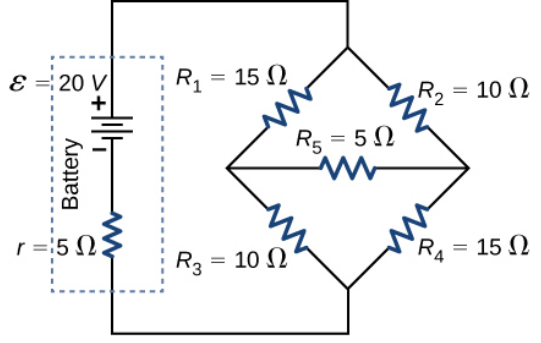
\includegraphics[width=0.4\textwidth]{circuit1.png}
\caption{\label{fig:circuit1} A circuit with five resistors powered by a battery with internal resistance.}
\end{figure}
What is the current flowing from the battery in Fig. \ref{fig:circuit1}?  What is the total power consumption? \\ \textbf{The current from the battery is $I = 1.17$ A, and the total power consumption is 23.4 W.}
\item 
\begin{figure}[ht]
\centering
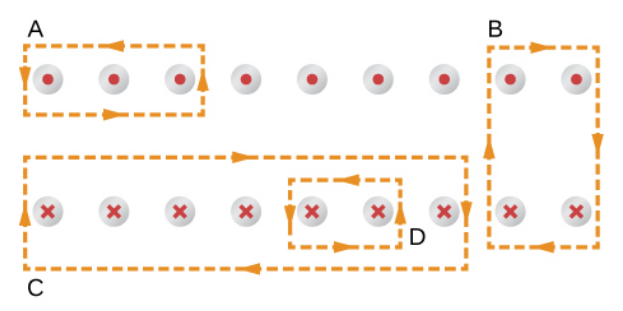
\includegraphics[width=0.4\textwidth]{circuit2.png}
\caption{\label{fig:circuit2} A circuit consisting of two batteries and five resistors.}
\end{figure}
Solve algebraiclly for the five currents in Fig. \ref{fig:circuit2}.  Remember to use the \textit{junction rule} and the \textit{loop rule.} \\ \textbf{Hint:}
\begin{itemize}
\item Loop 1: $I_1 R_1 - I_2 R_2 + V_1 = 0$
\item Loop 2: $I_2 R_2 + I_3 R_3 - I_4 R_4 - V_2 = 0$
\item Loop 3: $-I_5 R_5 + V_2 = 0$
\item Junction 1: $I_1 + I_3 = I_2$
\item Junction 2: $I_2 + I_5 = I_4$
\end{itemize}
\item 
\begin{figure}[ht]
\centering
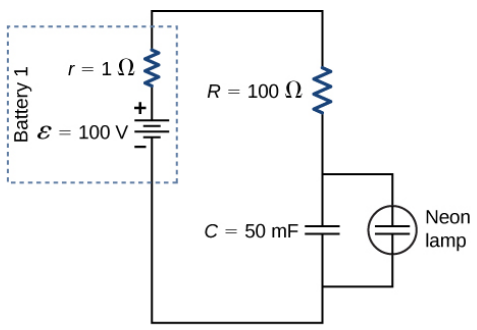
\includegraphics[width=0.3\textwidth]{circuit3.png}
\caption{\label{fig:circuit3} This type of circuit is called a relaxation oscillator.}
\end{figure}
Figure \ref{fig:circuit3} shows a \textit{relaxation oscillator}.  The RC circuit charges, and once the capacitor voltage reaches 50 V, the neon lamp lights and completely discharges the capacitor.  The process then repeats.  How long between neon lamp flashes? \\ Let $\tau = RC$.  \textbf{It can be shown that the voltage across the capacitor is given by}
\begin{equation}
V(t) = \epsilon\left(1 - \exp\left(-t/\tau\right)\right)
\end{equation}
We solve for the time:
\begin{equation}
t = -\tau \ln\left( 1 - V/\epsilon \right)
\end{equation}
Plugging in the numbers, we find that each 3.5 seconds, the voltage will be 50 V.  Thus, the lamp flashes every 3.5 seconds.
\end{enumerate}
\item \textbf{Chapter 11: Magnetic forces and fields}
\begin{enumerate}
\item 
\begin{figure}[ht]
\centering
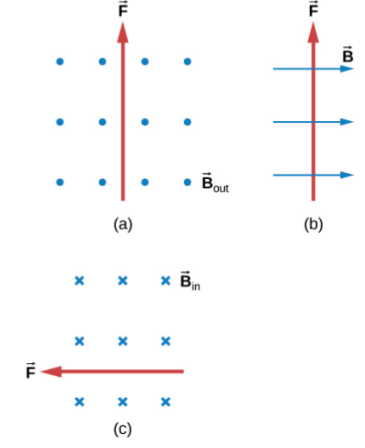
\includegraphics[width=0.3\textwidth]{lorentz1.png}
\caption{\label{fig:lorentz1} Each diagram depicts the force on a negatively-charged particle in a B-field.}
\end{figure}
Determine the velocity of a negatively-charged particle in Fig. \ref{fig:lorentz1} (a)-(c). \\ \begin{itemize}
\item (a): To the right.
\item (b): In to the page.
\item (c): Down.
\end{itemize}
\item A cosmic-ray electron moves at $6 \times 10^6$ m/s perpendicular to Earth’s magnetic field at an altitude where the field strength is $1.0 \times 10^{-5}$ T. What is the radius of the circular path the electron follows?  Show that the \textit{angular velocity} $\omega$ of the electron around the magnetic field lines is related to the $q/m$ ratio by $\omega/B = q/m$. \\ \textbf{We find the radius by setting the Lorentz force equal to the centripetal force.}
\begin{equation}
r = \frac{mv}{qB}
\end{equation}
\textbf{The result turns out to be $\approx 3.4$ m.}
\item What is the maximum torque on a 150-turn circular loop of wire with radius 8.0 cm that carries a 50.0-A current in a 1.60 T B-field? \\ \textbf{The simplified formula turns out to be}
\begin{equation}
\tau = N I A B = 150 \times 50 \times \pi \times 0.08^2 \times 1.6 \approx 240
\end{equation}
\textbf{Thus, 240 N m of torque.}
\end{enumerate}
\item \textbf{Chapter 12: Sources of Magnetic Fields}
\begin{enumerate}
\item What is the magnetic field created by the loops in the previous problem, at the center of the loops?  What is the \textit{total} magnetic moment of the loops? \\ 
\textbf{The magnetic field formula follows from the Biot-Savart law:}
\begin{equation}
B = \frac{N \mu_0 I}{2R} = \frac{150 \times 4\pi \times 10^{-7} \times 50.0}{2 \times 0.08} \approx 590 G
\end{equation}
\textbf{About 590 Gauss.}
\item Using Amp\`{e}re's Law, re-derive the equation for a magnetic field due to a long staight wire.  Now model a lightning bolt as a long straight wire.  A typical current in a lightning bolt is $10^4$ A. Estimate the magnetic field 1 m from the bolt. \\ \textbf{$BS = \mu_0 I$, so}
\begin{equation}
B = \frac{\mu_0 I}{S} =  \frac{\mu_0 I}{2 \pi R}
\end{equation}
\textbf{Using the right hand rule gives the direction.  Plugging in the numbers, we find about 20 Gauss.}
\item
\begin{figure}
\centering
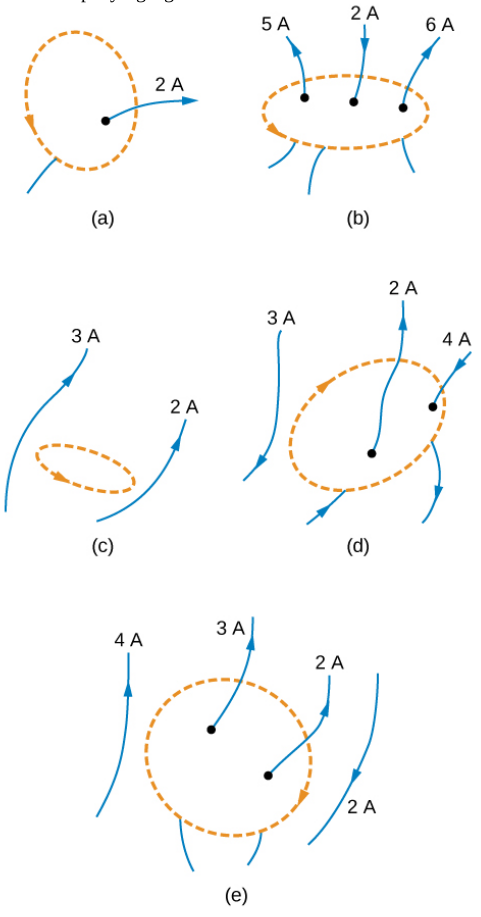
\includegraphics[width=0.3\textwidth,trim=0cm 0cm 0cm 0.25cm,clip=true]{amplaw.png}
\caption{\label{fig:amplaw} Several current arrangements with closed line integrals.}
\end{figure}
Evaluate $\oint \vec{B} \cdot d\vec{l}$ for cases (a)-(e) in Fig. \ref{fig:amplaw}. \\ \textbf{The basic concept of Ampere's Law is that this integral is proportional to the total enclosed current.  The constant of proportionality is $\mu_0$.}
\end{enumerate}
\end{enumerate}
\end{document}